\subsubsection{RoBERTa-Twitter Results}

The first step in fine-tuning RoBERTa-Twitter was to evaluate its performance without training the classification head and using the default weights, aiming to establish a baseline. Doing so yielded the classification report shown in Table~\ref{tab:classification_report_1} and the confusion matrix presented in Figure \ref{fig:confusion_matrix_roberta_shapeY_no_head}.

\begin{table}[H]
\centering
\caption{Classification Report without Training the Classification Head}
\label{tab:classification_report_1}
\begin{tabular}{lcccc}
\toprule
Class        & Precision & Recall & F1-score & Support \\
\midrule
0.0          & 0.00      & 0.00   & 0.00     & 3456    \\
1.0          & 0.52      & 1.00   & 0.68     & 3699    \\
\midrule
Accuracy     &           &        & 0.52     & 7155    \\
Macro Avg    & 0.26      & 0.50   & 0.34     & 7155    \\
Weighted Avg & 0.27      & 0.52   & 0.35     & 7155    \\
\bottomrule
\end{tabular}
\end{table}

\begin{figure}[H]
    \centering
    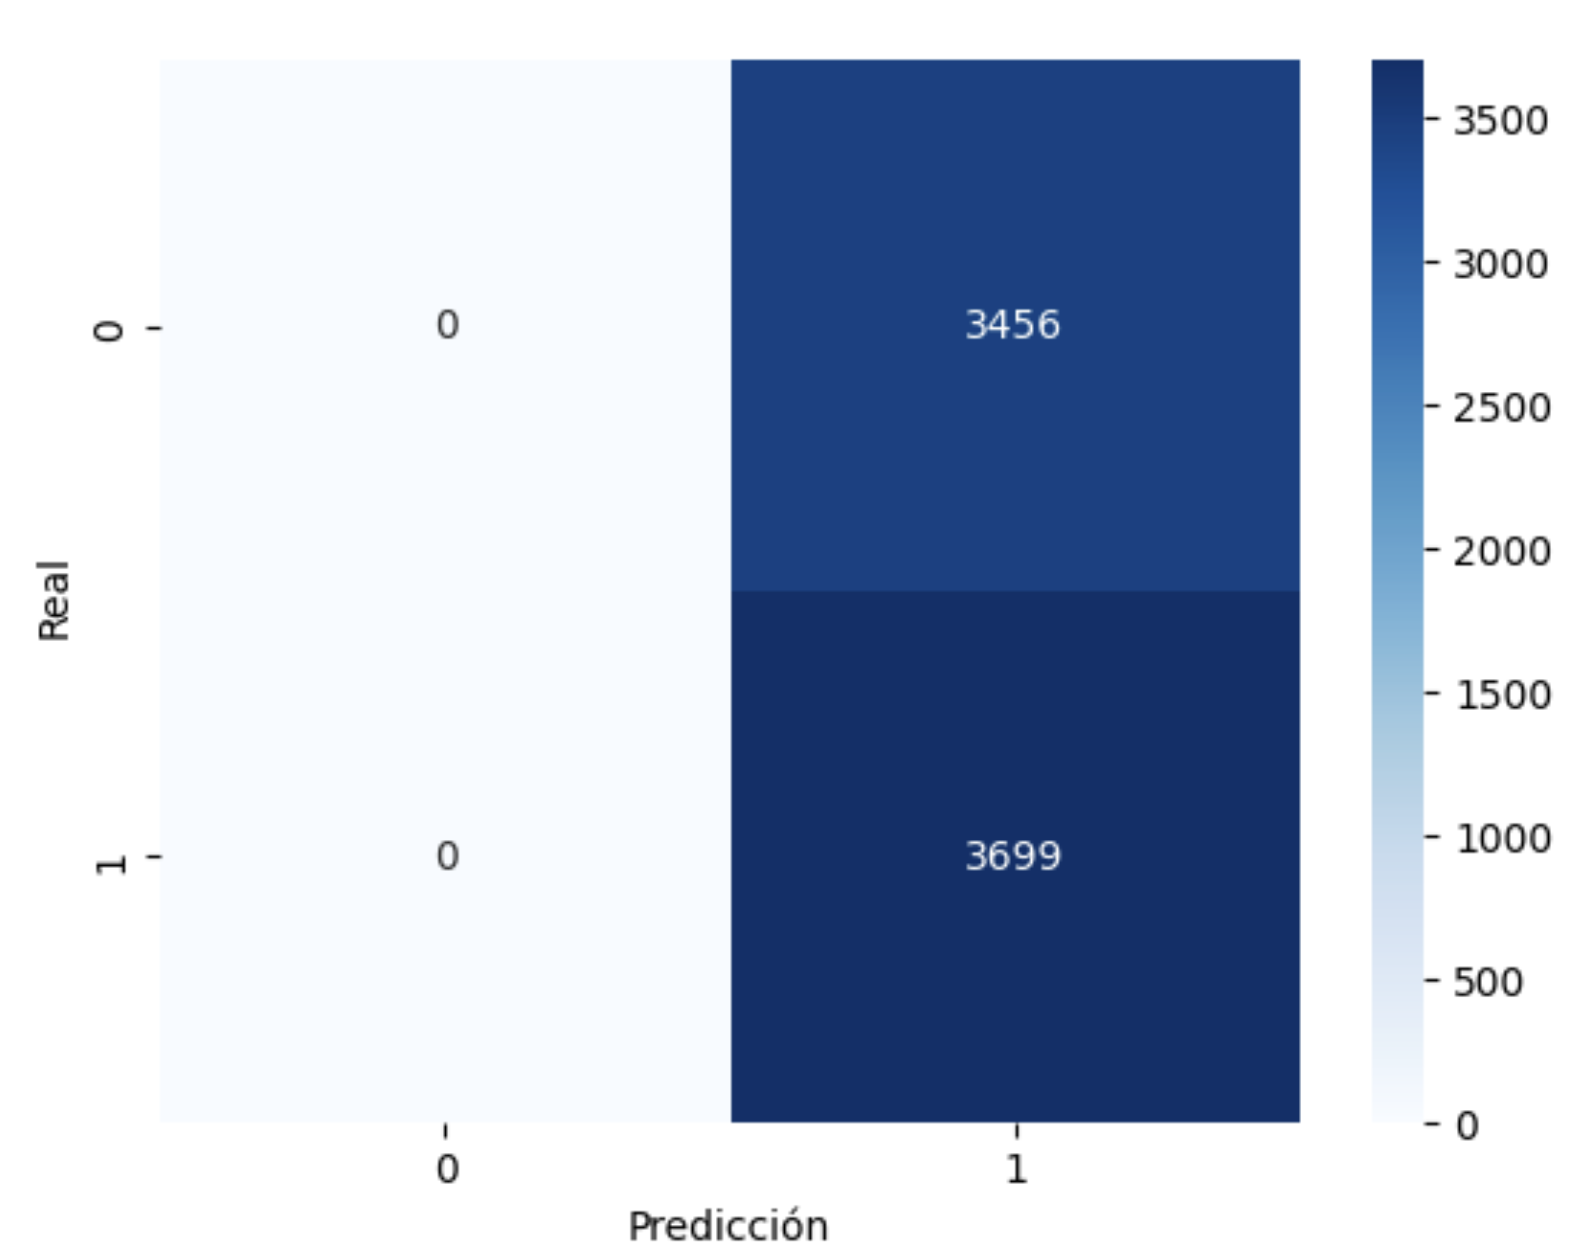
\includegraphics[width=0.45\textwidth]{images/confusion_matrix_bilstm_shapeY.png}
    \caption{RoBERTa-Twitter model confusion matrix without training the classification head}
    \label{fig:confusion_matrix_roberta_shapeY_no_head}
\end{figure}


As observed, the model predicts everything as toxic. This is because the classification head still retains its random weights and the RoBERTa-Twitter model has not yet been fine-tuned for this specific task.

Following the methodology, in the first training phase only the classification head is trained for 150 epochs. The results of this phase can be seen in Figures \ref{fig:roberta_validation_loss_finetune} and \ref{fig:roberta_accuracy_finetune}.


\begin{figure}[H]
    \centering
    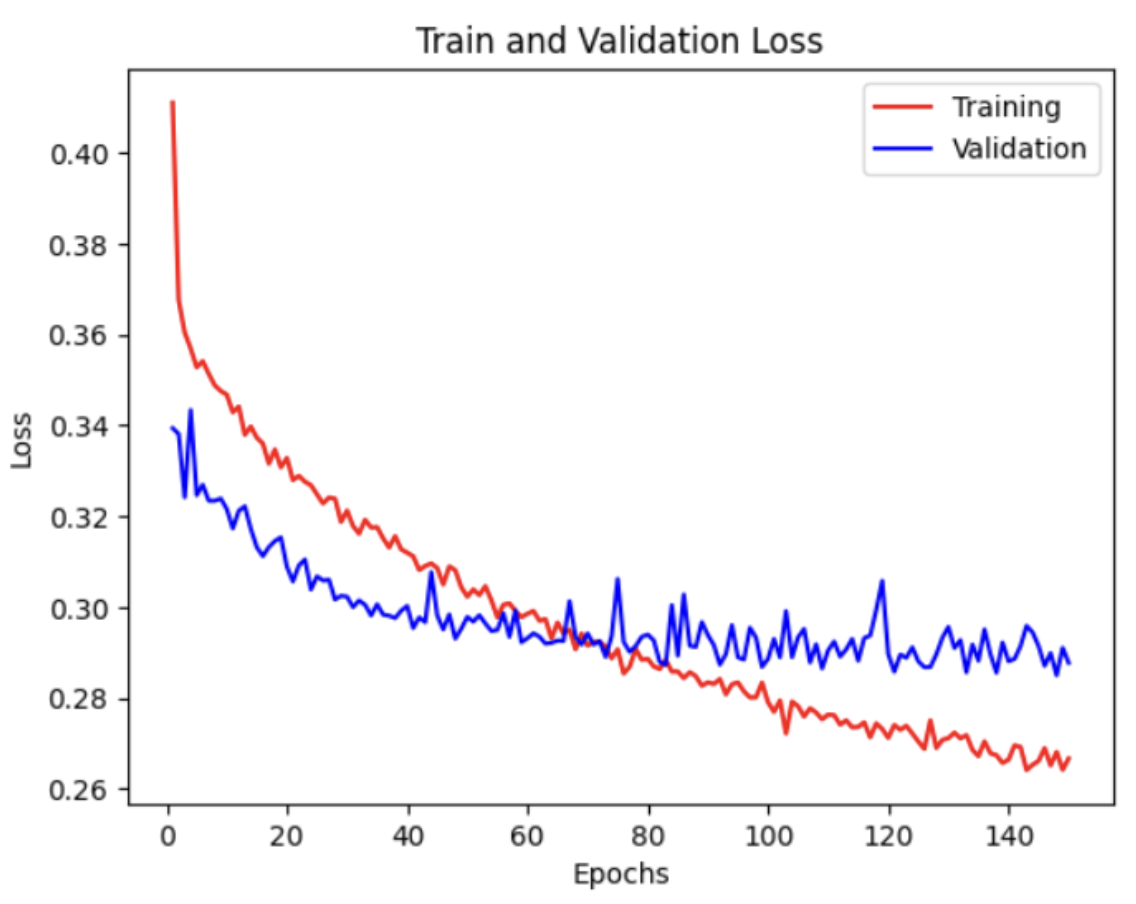
\includegraphics[width=0.45\textwidth]{images/robertaValidationLossFigureX15Epoch.png}
    \caption{Validation loss of the RoBERTa-Twitter model during classification head training (150 epochs)}
    \label{fig:roberta_validation_loss_finetune}
\end{figure}

\begin{figure}[H]
    \centering
    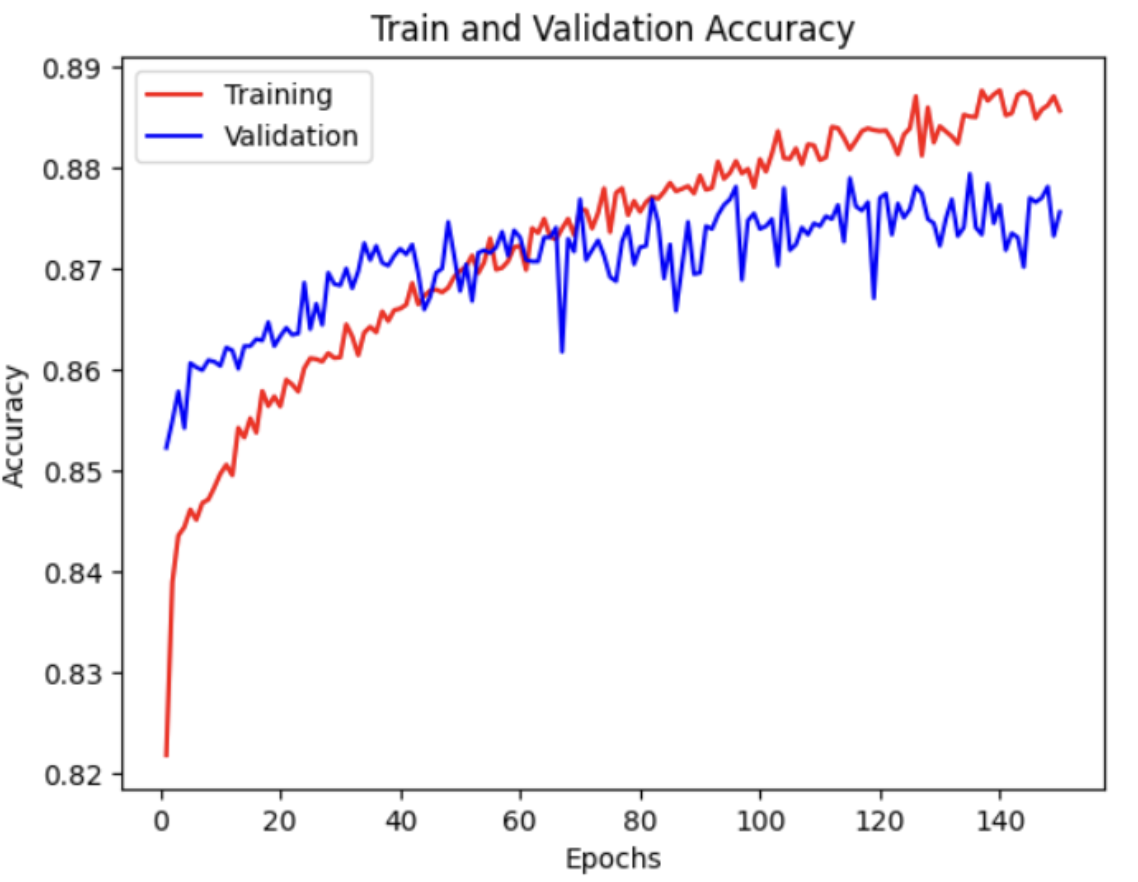
\includegraphics[width=0.45\textwidth]{images/robertaAccuracyFigureY150Epoch.png}
    \caption{Training and validation accuracy of the RoBERTa-Twitter model during classification head training}
    \label{fig:roberta_accuracy_finetune}
\end{figure}



Regarding the loss, it can be observed that around epoch 70, overfitting begins, as the validation loss stops decreasing or even starts to increase, while the training loss continues to drop rapidly. 

Concerning accuracy, it is noticeable that around epoch 70, the validation accuracy plateaus, whereas the training accuracy continues to improve. 

In summary, on the validation set, the loss stabilizes around 0.3 and the accuracy around 0.875, exhibiting an oscillatory behavior. The best validation accuracy was reached at epoch 135, with a value of 0.87937.

\begin{table}[H]
\centering
\caption{Classification Report after Training the Classification Head}
\label{tab:classification_report_2}
\begin{tabular}{lcccc}
\toprule
Class        & Precision & Recall & F1-score & Support \\
\midrule
0.0          & 0.85      & 0.91   & 0.88     & 3462    \\
1.0          & 0.91      & 0.84   & 0.88     & 3693    \\
\midrule
Accuracy     &           &        & 0.88     & 7155    \\
Macro Avg    & 0.88      & 0.88   & 0.88     & 7155    \\
Weighted Avg & 0.88      & 0.88   & 0.88     & 7155    \\
\bottomrule
\end{tabular}
\end{table}

\begin{figure}[H]
    \centering
    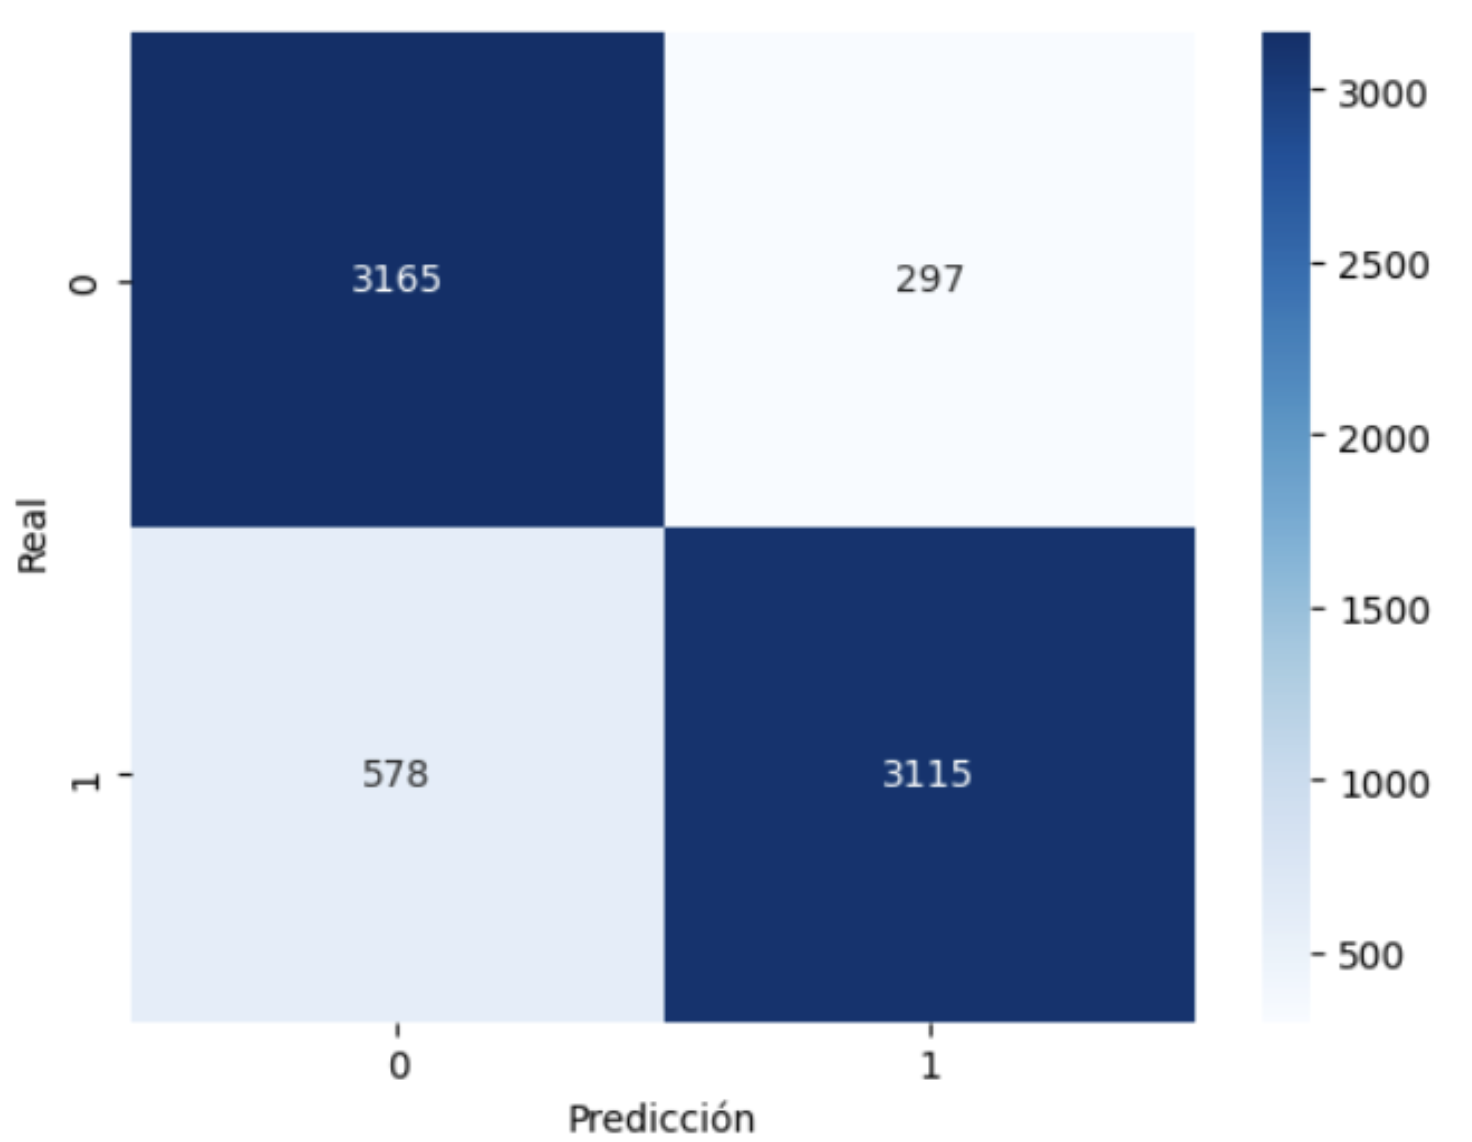
\includegraphics[width=0.45\textwidth]{images/robertaConfusionMatrix.png} 
    \caption{Confusion matrix of the RoBERTa-Twitter model}
    \label{fig:roberta_confusion_matrix}
\end{figure}

In previos charts, the classification report from the first training stage is shown. This report once again reflects a pattern observed in other models: low precision for the negative class, which results in low recall for the positive class. 

However, a surprising accuracy of 88\% was achieved by training only the designed classification head. This is supported by the confusion matrix in Figure X, where a high concentration of correct predictions and a reduced number of errors can be observed.

Based on the results from the first training phase, the model with the best validation accuracy was selected for the second stage. In this phase, all weights were unfrozen, and training continued for 100 epochs, saving the best-performing model.


\begin{figure}[H]
    \centering
    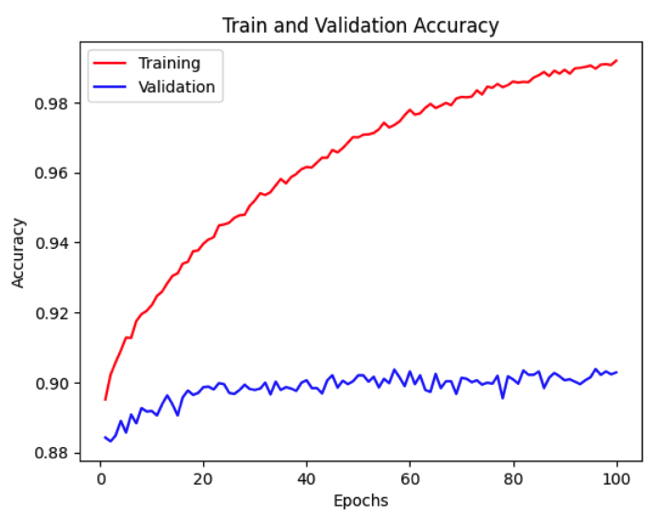
\includegraphics[width=0.45\textwidth]{images/robertaValidationAccuray100Epoch.png}
    \caption{Validation accuracy of the RoBERTa-Twitter model during full fine-tuning (100 epochs)}
    \label{fig:roberta_validation_accuracy_100epoch}
\end{figure}

\begin{figure}[H]
    \centering
    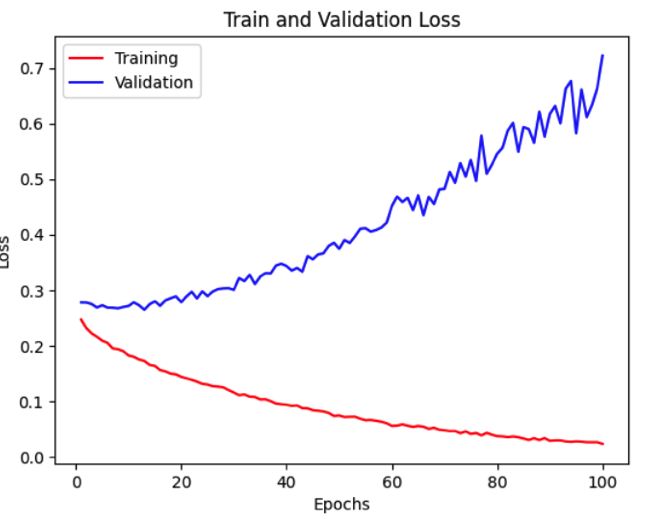
\includegraphics[width=0.45\textwidth]{images/robertaValidationLost100Epoch.png}
    \caption{Validation loss of the RoBERTa-Twitter model during full fine-tuning (100 epochs)}
    \label{fig:roberta_validation_loss_100epoch}
\end{figure}

Figures \ref{fig:roberta_validation_accuracy_100epoch} and \ref{fig:roberta_validation_loss_100epoch} show the evolution of loss and accuracy over the 100 training epochs. Overfitting can be observed in both loss and accuracy: the model continues to improve on the training set while deteriorating on the validation set. 

The validation loss increases rapidly, while the validation accuracy decreases more gradually. Nevertheless, the performance on the validation set improved, reaching a validation accuracy of 0.90383 at epoch 96.

\begin{table}[H]
\centering
\caption{Classification Report after Full Fine-Tuning}
\label{tab:classification_report_final}
\begin{tabular}{lcccc}
\toprule
Class        & Precision & Recall & F1-score & Support \\
\midrule
0.0          & 0.88      & 0.93   & 0.90     & 3462    \\
1.0          & 0.93      & 0.88   & 0.91     & 3693    \\
\midrule
Accuracy     &           &        & 0.90     & 7155    \\
Macro Avg    & 0.91      & 0.91   & 0.90     & 7155    \\
Weighted Avg & 0.91      & 0.90   & 0.90     & 7155    \\
\bottomrule
\end{tabular}
\end{table}


\begin{figure}[H]
    \centering
    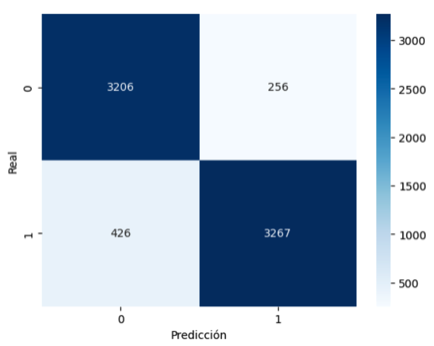
\includegraphics[width=0.45\textwidth]{images/robertaConfusionMatrix100Epochs.png} 
    \caption{Confusion matrix of the RoBERTa-Twitter model after full fine-tuning (100 epochs)}
    \label{fig:roberta_confusion_matrix_100epochs}
\end{figure}

As shown in Table \ref{tab:classification_report_final} and Figure \ref{fig:roberta_confusion_matrix_100epochs}, both the classification report and the confusion matrix are presented. These results reveal the issue of bias toward the negative class, a pattern seen in previous models. 

Nevertheless, the model achieves a remarkable performance of 90\% accuracy, which could be considered a potential solution to the problem. However, this result, while close, does not surpass the 92.38\% reported in \cite{fieri2023offensive}.
